% This Source Code Form is subject to the terms of the Mozilla Public
% License, v. 2.0. If a copy of the MPL was not distributed with this
% file, You can obtain one at https://mozilla.org/MPL/2.0/.

\documentclass[a4paper, 12pt]{article}

\usepackage[english, russian]{babel}
\usepackage[T2A]{fontenc}
\usepackage[utf8]{inputenc}
\setlength{\parindent}{1cm}
\usepackage{graphicx}
\usepackage{amsmath}
\usepackage{booktabs}
\usepackage{siunitx}
\usepackage{wrapfig}
\usepackage{siunitx}

\begin{document}
	
	\begin{center}
		\subsubsection*{Отчёт к лабораторной работе №162}
		
		\subsubsection*{"Исследование свойств полосовых фильтров"}
		
		\subsubsection*{Преподаватель: Петриков В. Д.}
		
		Выполнил студент третьего курса вышей школы фундаментальных физический исследований: Куликовских Илья
		
		Группа: 5030302/30801
	\end{center}
	
	\quad \textbf{1. Исследование свойств полосового RC-фильтра.}
	
	\quad 1.1. На монтажной плате нами была собрана схема полосно-пропускающего RC-фильтра с использованием двух одинаковых пар резисторов и конденсаторов. В качестве источника был подключен генератор переменного тока, осциллограф и миллифольтметры (рис. 1).
	
	\begin{figure}[h!]
		\centering
		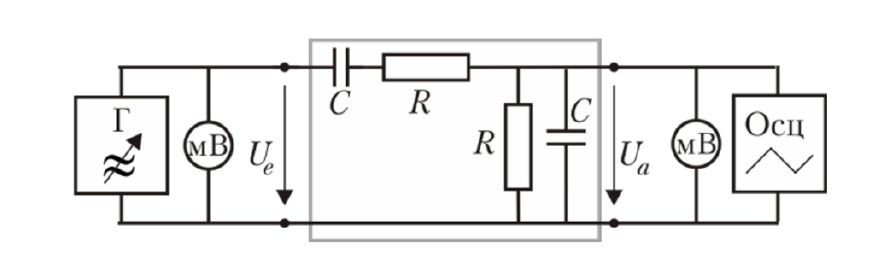
\includegraphics[width=0.8\textwidth]{RCfilt.png}
		\caption{Полосно-пропускающий $RC$-фильтр с подключенными приборами}
	\end{figure}
	
	\quad Определим теоретическое значение квазирезонансной частоты:
	
	\begin{center}
		$f_0 = \dfrac{1}{2\pi R C}$ 
		
		$f_0 = \dfrac{1}{2 \pi \cdot 51 \cdot 10^3 \cdot 1300 \cdot 10^{-12} } \approx 2400$ Гц $ = 2.4$ кГц
	\end{center}
	
	\quad Коэффициент передачи исследуемого фильтра $K = \dfrac{1}{3}$ B $ = 0.316$ В. 
	
	\quad 1.2. Для наблюдения резонанса мы перевели осциллограф в режим XY и затем ожидали прямой линии на экране, при этом варьируя значение частоты на генераторе. В результате эксперимента резонансная частота имеет значение: $f_0 = 2.32$ кГц. Причина, по которой мы наблюдаем именно прямую линию, заключается в том, что при совпадении частот, напряжение собственных колебаний выражается через напряжение вынуждающей силы с точностью до постоянного коэфицента (отношения амплитуд), следовательно мы наблюдаем линейную зависимость (рис. 2). 
	
	\begin{wrapfigure}[12]{r}{0.5\textwidth}
		\centering
		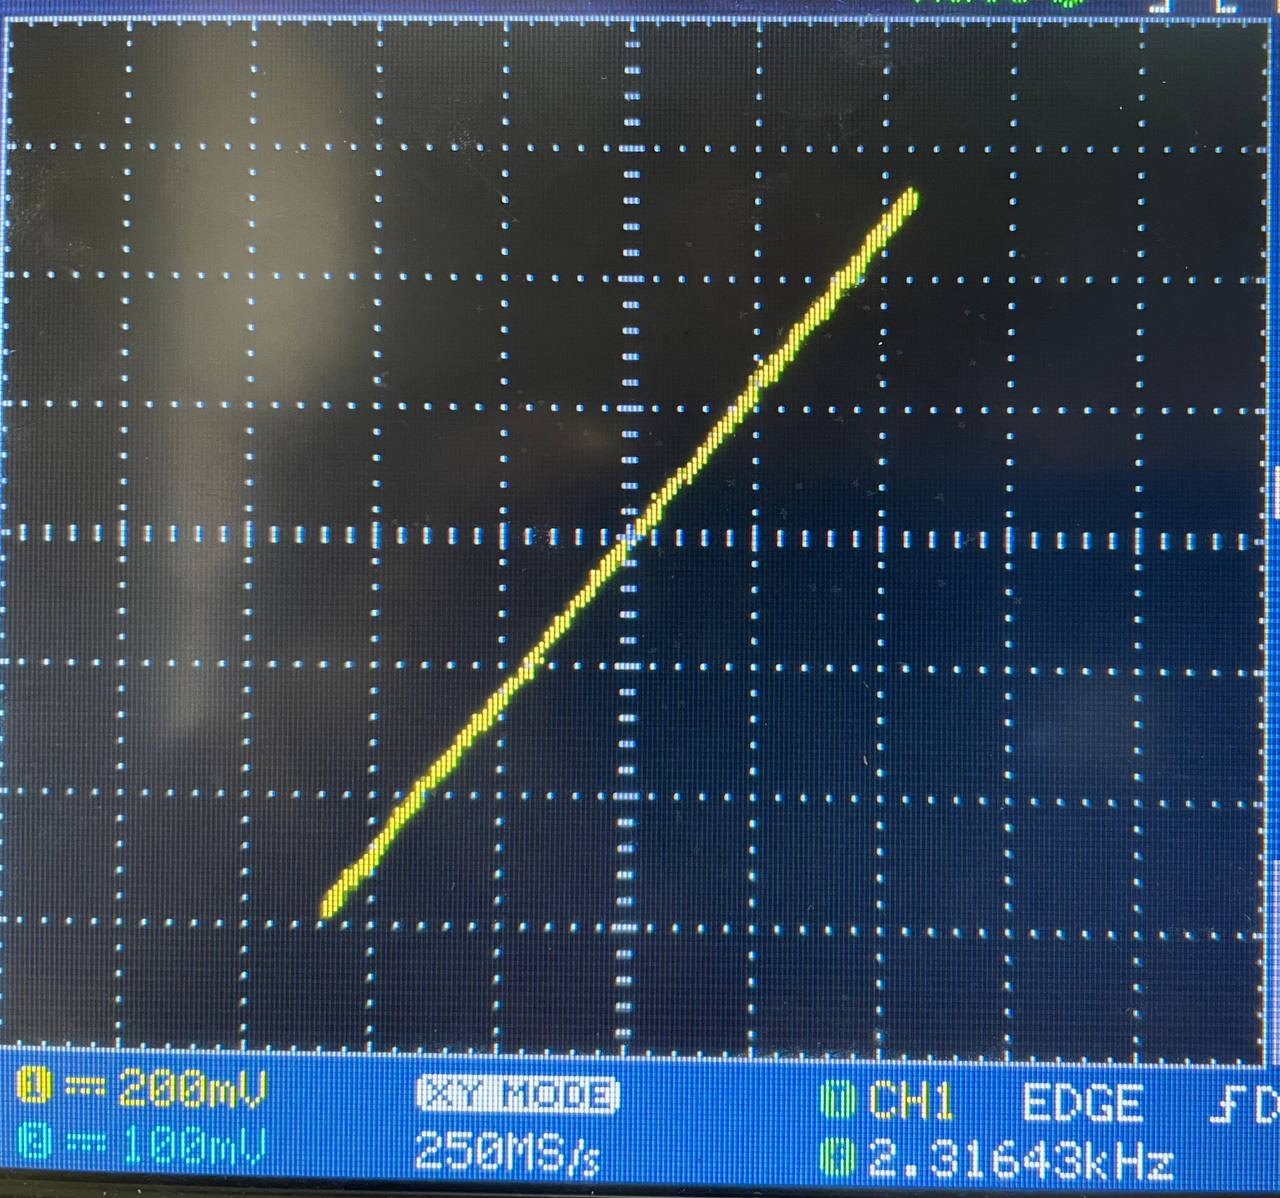
\includegraphics[width=0.4\textwidth]{resline.jpg}
		\caption{форма фигуры Лиссажу при резонансе}
	\end{wrapfigure}
	
	\quad Ниже в таблице приведены результаты измерения напряжения в зависимости от чстоты для расчёта значения полосы пропускания фильтра. По данным таблицы ширина полосы пропускания добротность составляют: 
	
	\begin{center}
		$\Delta f = 5.1$ кГц. 
		
		$Q = 0.4549 $
	\end{center}
	
	\quad По результатам эксперимента погрешность определения резонансной частоты составляет меньше одного процента.
	
	\begin{table}[h!]
		\caption{Зависимость выходного напряжения от частоты}
		\label{tab:voltage_frequency}
		\begin{tabular}{c|c|c}
			\toprule
			\textbf{Частота, кГц} & \textbf{Входное напряжение, В} & \textbf{Выходное напряжение, В} \\
			\midrule
			2,32 & 9.5 & 3.00 \\ \hline
			1,00 & 9.5 & 2.12 \\ \hline
			6,10 & 9.5 & 2.12 \\
			\bottomrule
		\end{tabular}
	\end{table}

	\quad 1.3. Далее генератор был переведён в режим генерации прямоугольных импульсов напряжения. Осцилограмма переходной характеристики фильтра выглядит следующим образом (рис. 3). 
	
	\begin{figure}[htbp]
		\centering
		\begin{minipage}{0.45\textwidth}
			\centering
			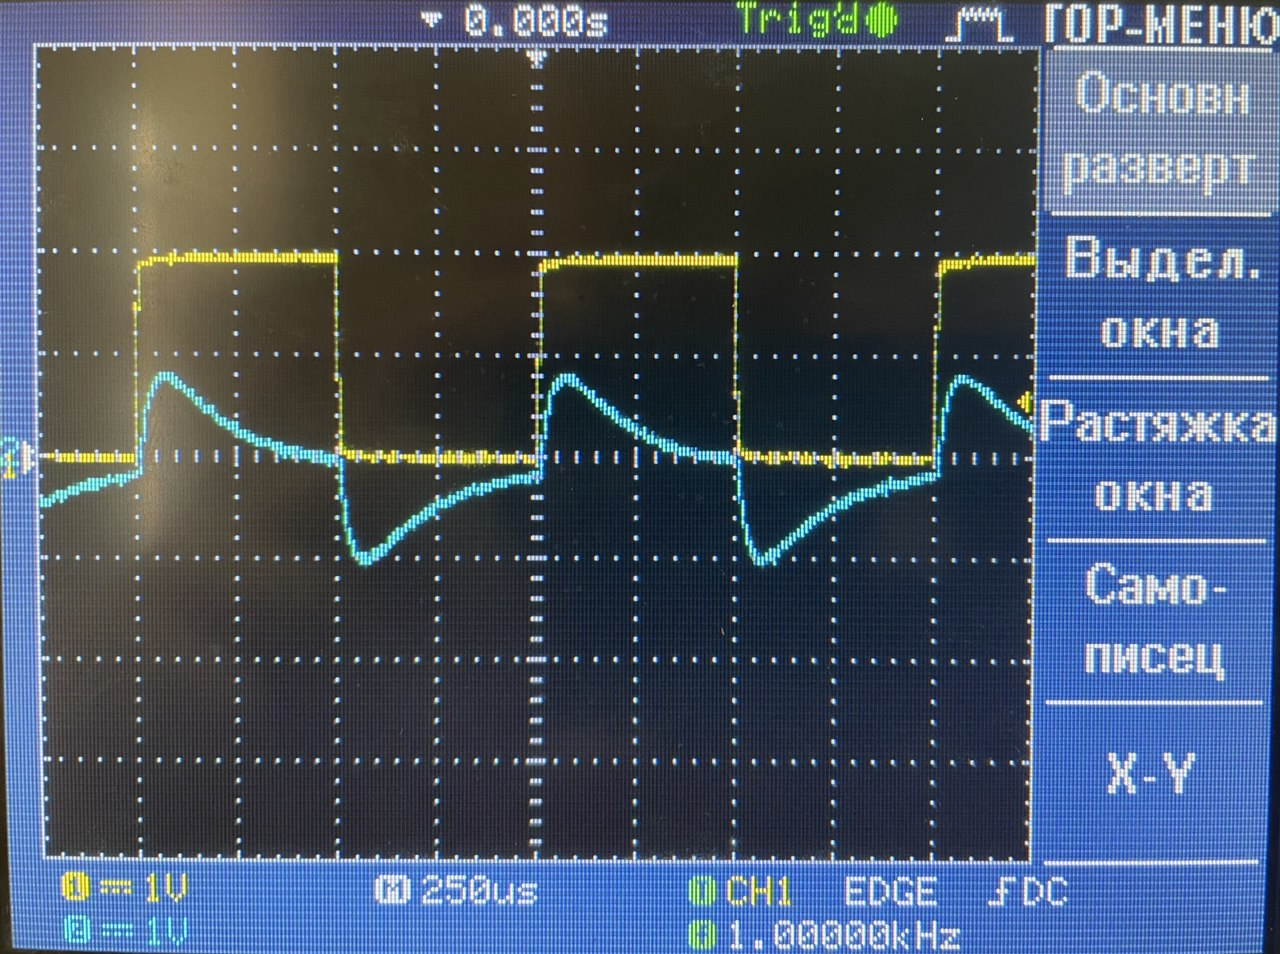
\includegraphics[width=0.9\linewidth]{charecterfilt.jpg}
			\caption{Экспериментальная переходная характеристика RC-фильтра}
			\label{fig:exp_char}
		\end{minipage}
		\hfill
		\begin{minipage}{0.45\textwidth}
			\centering
			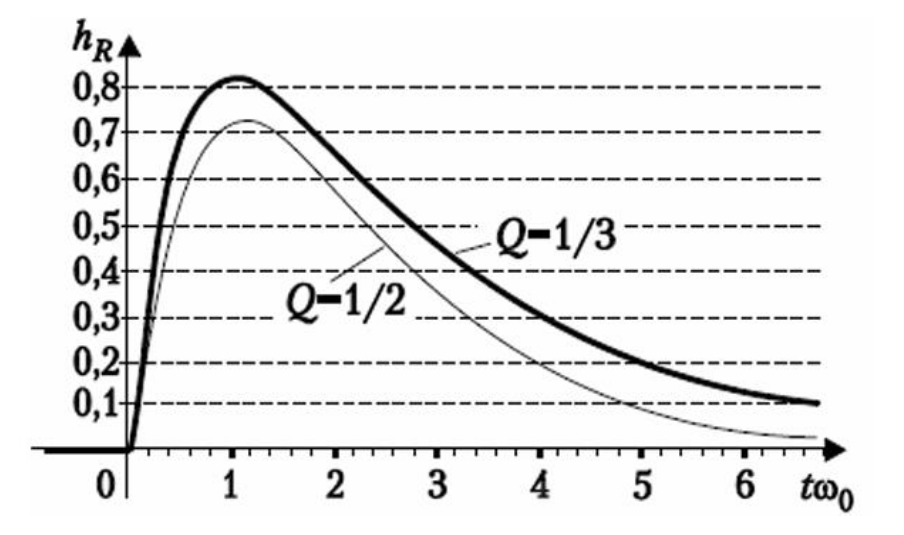
\includegraphics[width=1.0\linewidth]{characterfilt_teor.png}
			\caption{Теоретическая переходная характеристика RC-фильтра}
			\label{fig:teor_char}
		\end{minipage}
	\end{figure}
	
	\quad График, наблюдаемый нами на осцилографе, полностью соотвествует приведённому графику переходной характеристики (рис. 4). 
	
	\quad \textbf{2. Анализ частотных свойств последовательного колебательного контура}
	
	\quad 2.1. Мы собрали последовательный колебательный контур используя катушку и конденсатор из набора (рис. 5).
	
	\begin{figure}[htbp]
		\centering
		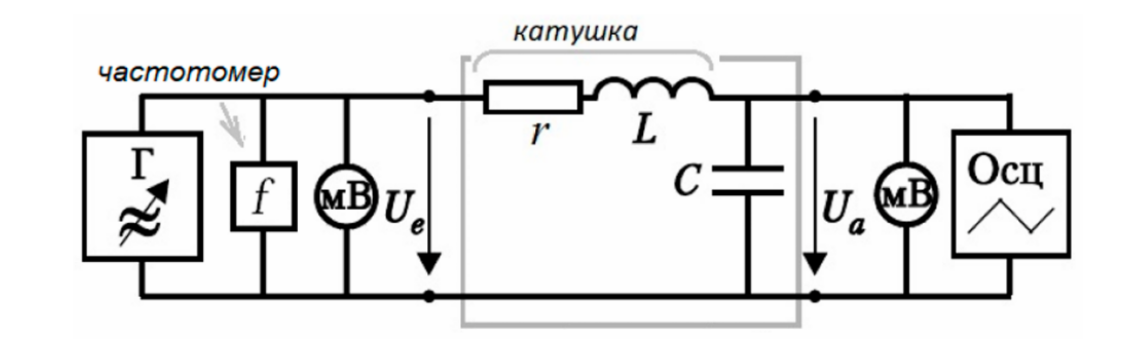
\includegraphics[width=0.9\linewidth]{cont.png}
		\caption{Схема колебательного контура}
	\end{figure}
	
	\quad Характеристики контура:
	
	\begin{center}
		$C = 10\,\text{нФ}$ \qquad $L = 750\,\text{мкГн}$
	\end{center}
	
	\quad Тогда квазирезонансная частота равна:
	
	\begin{center}
		$f = \dfrac{1}{2\pi\sqrt{LC}} = 58.115~\text{кГц}$.
	\end{center}
	
	\quad Результат экспериментального значения резонансной частоты:
	\[
	f_0 = 60.018 \text{кГц},
	\]
	
	\quad Проделав аналогичные действия с отношением $\dfrac{U_{\text{вых}}}{U_{\text{вх}}}$, определим добротность контура:
	\[
	Q = \frac{28}{0.95} = 29.474
	\]
	
	\quad Определим реальное $r$ (подставлены ваши числа):
	
	\begin{center}
		$Q = \dfrac{R_0}{\sqrt{L/C}},\qquad R = \dfrac{L}{C\,r}$
	\end{center}
	
	\begin{equation*}
		\begin{aligned}
			Q &= \frac{L}{C\,r\,\sqrt{L/C}}
			= \frac{1}{r}\sqrt{\frac{L}{C}}
			\quad\Longrightarrow\quad
			r = \frac{\sqrt{L/C}}{Q}.
		\end{aligned}
	\end{equation*}
	
	\begin{equation*}
		\begin{aligned}
			\sqrt{\frac{L}{C}} &= \sqrt{\frac{750\cdot10^{-6}}{10\cdot10^{-9}}}
			= 273.8612787,\\[4pt]
			r &= \frac{273.8612787}{29.474} = 9.283\ \text{Ом}.
		\end{aligned}
	\end{equation*}
	
	\quad 2.2. Проверим насколько экспериментальные данные отходят теорических: $\dfrac{58.115}{60.018} = 0.968$, т.е. экспериментальные данные отходят от теорических всего $3.2 \% $. 
	
	\[
	\begin{gathered}
		Q = \dfrac{2\pi f_0 L}{r} 
		= \dfrac{2\cdot 3.141592 \cdot 60.018\cdot 750\cdot10^{-6}}{9.283}
		= 30.467 \\[6pt]
		\dfrac{Q_{\text{э}}}{Q_{\text{т}}}
		= \dfrac{29.474}{30.467}
		= 0.967
	\end{gathered}
	\]
	
	
	\quad Таким образом погрешность в измерении добротности состовляет примерно $3.3\% $. 
	
	\quad  2.3.	Необходимо определить эволюцию добротности в зависимости от интенсивности подающего напряжения. Проведём измерения (Таблица 2. Результаты измерений). 
	
	\begin{table}[h!]
		\centering
		\begin{tabular}{ccccc}
			\toprule
			$f$ (кГц) & $U_{\text{вх}}$ (мВ) & $U_{\text{вых}}$ (мВ) & $f-\langle f\rangle$ & $(f-\langle f\rangle)^2$ \\
			\midrule
			59.87 & 4.5 & 84  & -0.14833333 & 0.022002778 \\
			60.60 & 5.5 & 105 &  0.58166667 & 0.338336111 \\
			61.30 & 6.0 & 110 &  1.28166667 & 1.642669444 \\
			58.92 & 7.0 & 130 & -1.09833333 & 1.206336111 \\
			59.45 & 8.0 & 145 & -0.56833333 & 0.323002778 \\
			59.97 & 9.0 & 160 & -0.04833333 & 0.002336111 \\
			\midrule
			$\dfrac{1}{n}\Sigma = 60.018$ & & & $\Sigma = -2.84\cdot 10^{-14}$ & $\Sigma = 3.53$ \\
			\bottomrule
		\end{tabular}
		\caption{Результаты измерений}
	\end{table}
	
	\begin{figure}[htbp]
		\centering
		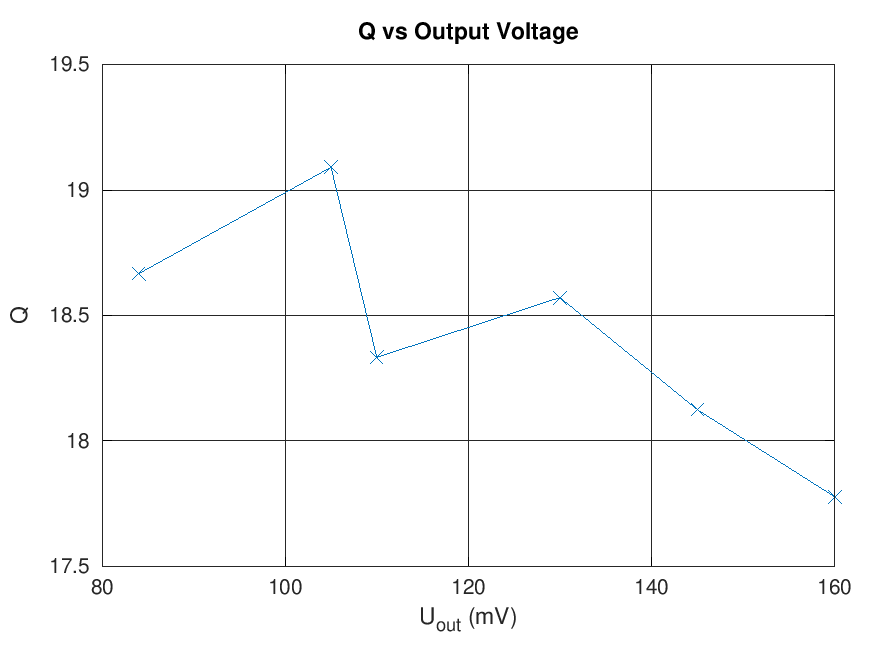
\includegraphics[width=0.76\linewidth]{Q_vs_Uout.png}
		\caption{Зависимость добротности от выходного напряжения}
	\end{figure}
	
	\begin{figure}[htbp]
		\centering
		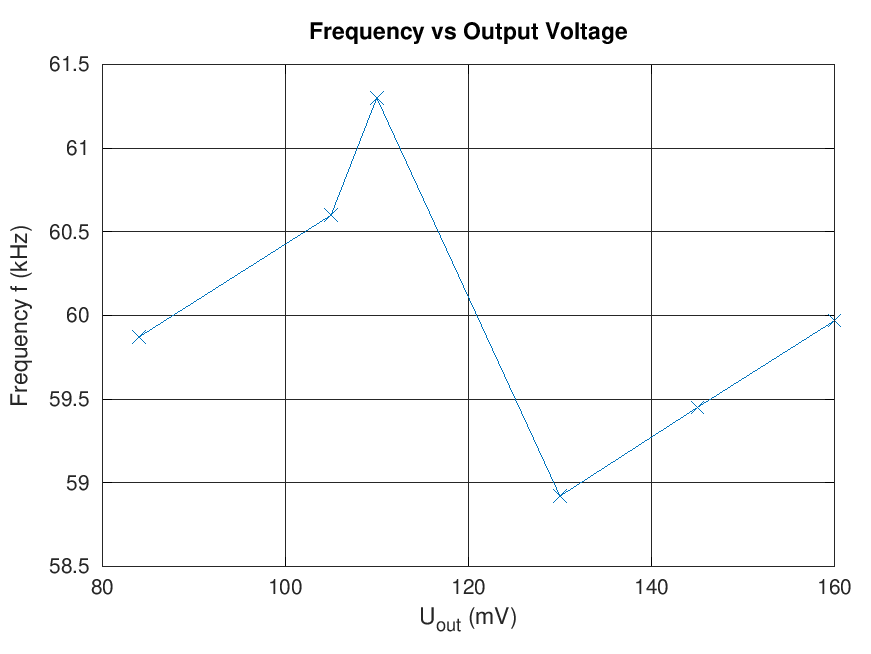
\includegraphics[width=0.76\linewidth]{frequency_vs_Uout.png}
		\caption{Зависимость резонансной частоты от выходного напряжения}
	\end{figure}
	
	
	\quad Из вида графиков (рис. 6 и рис. 7) можно сделать выводы о том, что добротность обратнопропорцианально зависит от выходного напряжения, а резонансная частота не имеет явной зависимости от выходного/входного напряжений. 
	
	\quad \textbf{3. Анализ свойств полосового LC-фильтра.} 
	
	\quad 3.1. Мы собрали полосовой фильтр, составив из катушки индуктивности и конденсатора параллельный колебательный контур с характеристиками: 
	
	\begin{center}
		$C = 10$ нФ, $L = 750$ мкГн 
		
		$R_g = 51$ кОм, $C_k = 150$ пФ  
	\end{center}
	
	\begin{figure}[htpb]
		\centering
		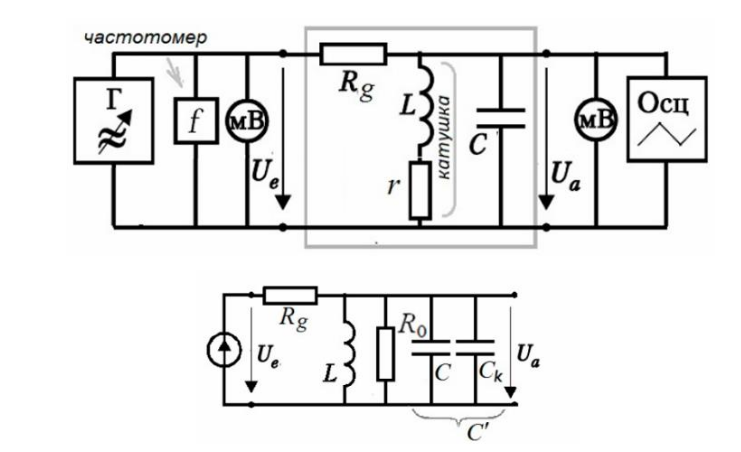
\includegraphics[width=0.7\linewidth]{LCfilt.png}
		\caption{Схема полосового LC-фильтра}
	\end{figure}
	
	\quad Экспериментальное значение резонансной частоты контура равно: 
	
	\begin{center} 
		$f_0 = 54.789$ кГц
	\end{center}
	
	\quad Входное и выходное значения напряжения равны соответсвенно: 
	
	\begin{center}
		$U_{\text{вх}} = 86$ мВ, $U_{\text{вых}} = 16$ мВ $\implies$
		
		$\implies R_0 = \dfrac{U_{\text{вых}} R_g}{U_{\text{вх}} - U_{\text{вых}}} = \dfrac{16 \cdot 10^{-3} \cdot 51 \cdot 10^{3} }{86 \cdot 10^{-3} - 16 \cdot 10^{-3}} = 11.657$ кОм 
	\end{center}
	
	\quad $R_0$ - это эквивалетное сопротивление на частоте резонанса. 
	
	3.2. Далее с помощью частотометра были измерены границы полосы пропускания: 
	
	\begin{center}
		$f_{\text{н}} = 53.815$ кГц, $f_{\text{в}} = 55.714$ кГц
	\end{center}
	
	\quad По значениям границы полосы пропускания вычислим добротность: 
	
	\begin{center}
		$Q_{\text{экс}} = \dfrac{f_0}{\Delta f} = 28.851$
	\end{center}
	
	3.3. Определим теоретические значения параметров системы: 
	
	\begin{center}
		$f_0 = \dfrac{1}{2\pi\sqrt{L(C + C_\kappa)}} $
		
		$f_0 = \dfrac{1}{2\pi\sqrt{750 \times 10^{-6} \cdot (10 \times 10^{-9} + 150 \times 10^{-12})}} = 57.68$ кГц 
	\end{center}
	
	\quad Погрешность в экспериментальном определении резонансной частоты составляет примерно $6 \%$. 
	
	3.4. К колебательному контуру был подсоединён генератор прямоугольного напряжения. На осцилографе мы наблюдали картину следующего вида (рис. 9). В процессе измерения были сняты пиковые(амплитудные) значения напряжения для определения инкрмента затухания. 
	
	\begin{figure}[htpb]
		\centering
		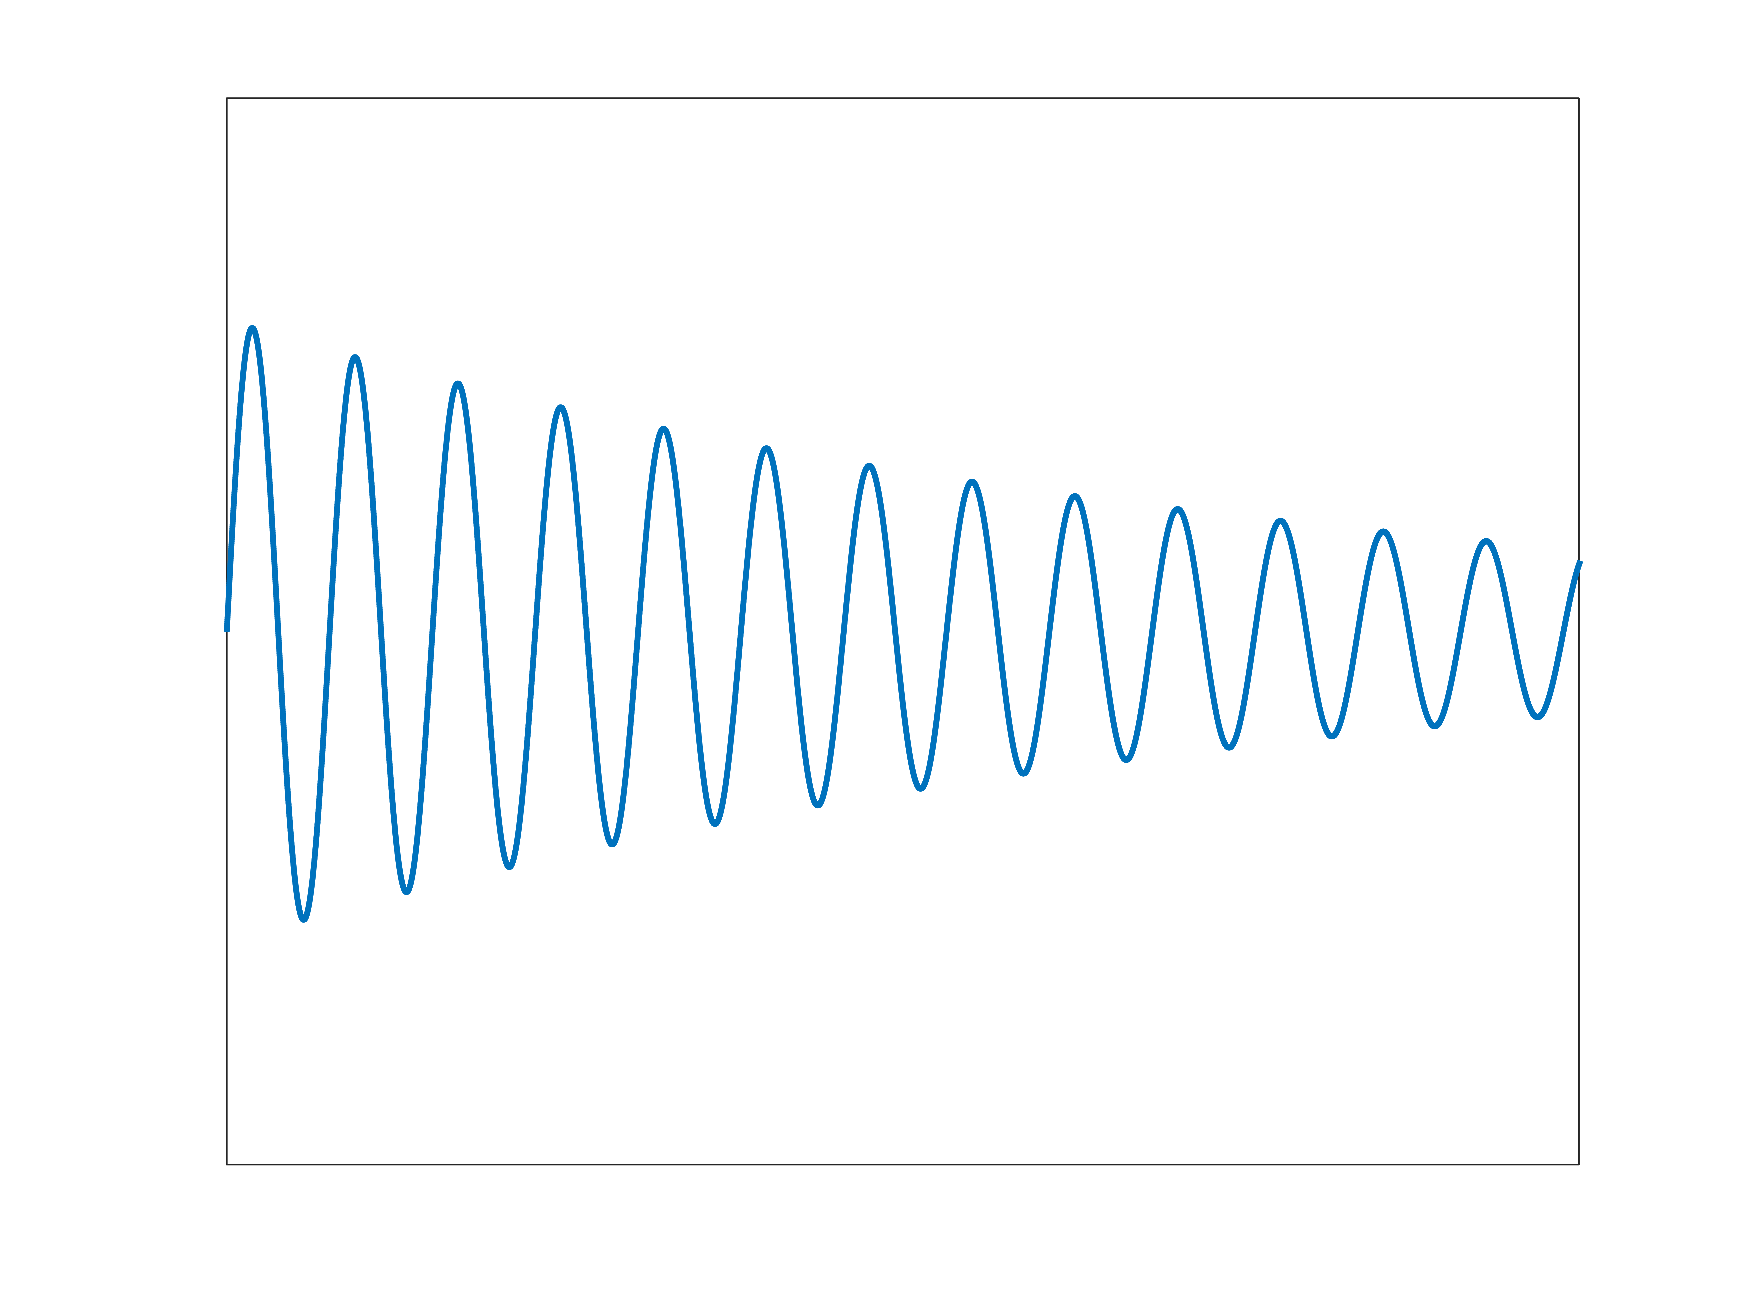
\includegraphics[width = 0.7\linewidth]{oscillogram.png}
		\caption{Отклик системы на прямоугольные напряжения}
	\end{figure}
	
	\quad Таким образом инткремент затухания и частота собственных колебаний соответственно равны: 
	
	\begin{center}
		$\beta = \left< \ln\dfrac{U_n}{U_{n+1}} \right> = 0.101$
		
		$f = \dfrac{1}{T} = \dfrac{1}{19\cdot10^{-6}} = 52.632$ кГц
	\end{center}
	
	3.5. По результатам измерения инкремента затухания и полосы пропускания определим нагруженную добротность и частоту резонанса: 
	
	\begin{center}
		$$Q = \dfrac{\pi}{\beta} = 31.1 $$
	
		$f = 52.632$ кГц 
	\end{center}
	
	\quad Теоретическое значение добротности отличается от экспериментального в пределах 10\%. 
	
	\quad \textbf{Выводы: }
	
	В ходе лабораторной работы были исследованы три типа фильтров: полосовой RC-фильтр, последовательный колебательный контур и полосовой LC-фильтр.
	
	При изучении RC-фильтра теоретическое значение квазирезонансной частоты составило $f_0 = 2400$ Гц, тогда как экспериментальное значение оказалось равным $f_{0\text{экс}} = 2320$ Гц. Расхождение составляет 3.3\%, что находится в пределах допустимой погрешности радиоэлементов. Добротность фильтра $Q = 0.455$ соответствует низкодобротной системе, что характерно для RC-цепей.
	
	Для последовательного колебательного контура экспериментальная резонансная частота $f_{0\text{экс}} = 60.018$ кГц хорошо согласуется с теоретическим значением $f_0 = 58.115$ кГц (отличие 3.2\%). Добротности $Q_{\text{теор}} = 30.467$ и $Q_{\text{экс}} = 29.474$ также демонстрируют хорошее соответствие с погрешностью 3.3\%.
	
	В случае LC-фильстра экспериментальная резонансная частота $f_{0\text{экс}} = 54.789$ кГц несколько отличается от расчетной $f_0 = 57.68$ кГц (погрешность 5.3\%). Нагруженная добротность, определенная через полосу пропускания, составила $Q_{\text{экс}} = 28.851$, а по затуханию колебаний $Q = 31.1$. Анализ переходного процесса позволил определить декремент затухания $\beta = 0.101$ и частоту собственных колебаний $f = 52.632$ кГц.
	
	Таким образом, экспериментальные данные в основном подтверждают теоретические расчеты. Наибольшие расхождения наблюдаются для LC-фильтра, что может быть связано с паразитными параметрами элементов и влиянием измерительной аппаратуры. Высокая добротность колебательных контуров (порядка 30) обеспечивает хорошую избирательность по сравнению с RC-фильтром, что подтверждается существенно более узкой полосой пропускания.
	
\end{document}